
\begin{frame}{Leiblein (Gumbel Approximation) New Orleans}
\vspace{-20pt}
    %\centering
 \begin{minipage}{1.0\textwidth}
\begin{figure}[htb!]
    \centering
    \includegraphics[width=1\linewidth]{../surge/plots/Lieblein_modelNO.pdf}
    \vspace{-15pt}
   \caption{Interesting transition - does this represent hurricanes? }
    \label{fig:}
\end{figure}
\end{minipage}
\end{frame}


\begin{frame}{Leiblein (Gumbel Approximation) Miami}
\vspace{-20pt}
 \begin{minipage}{1.0\textwidth}
\begin{figure}[htb!]
    \centering
    \includegraphics[width=1\linewidth]{../surge/plots/Lieblein_modelMM.pdf}
    \vspace{-15pt}
   \caption{Fits Line well. }
    \label{fig:}
\end{figure}
\end{minipage}
\end{frame}


\begin{frame}{Leiblein (Gumbel Approximation) Along Coast}
\vspace{-20pt}
    %\centering
 \begin{minipage}{1.0\textwidth}
\begin{figure}[htb!]
    \centering
    \includegraphics[width=1\linewidth]{../surge/plots/skextreme_first_tactic.pdf}
    \vspace{-15pt}
   \caption{. }
    \label{fig:}
\end{figure}
\end{minipage}
\end{frame}




\section{Tauuo, $\tau_u$ }
    \begin{frame}[plain]
        \vfill
      \centering
      \begin{beamercolorbox}[sep=8pt,center,shadow=true,rounded=true]{title}
        \usebeamerfont{title}\insertsectionhead\par%
        \color{oxfordblue}\noindent\rule{10cm}{1pt} \\
                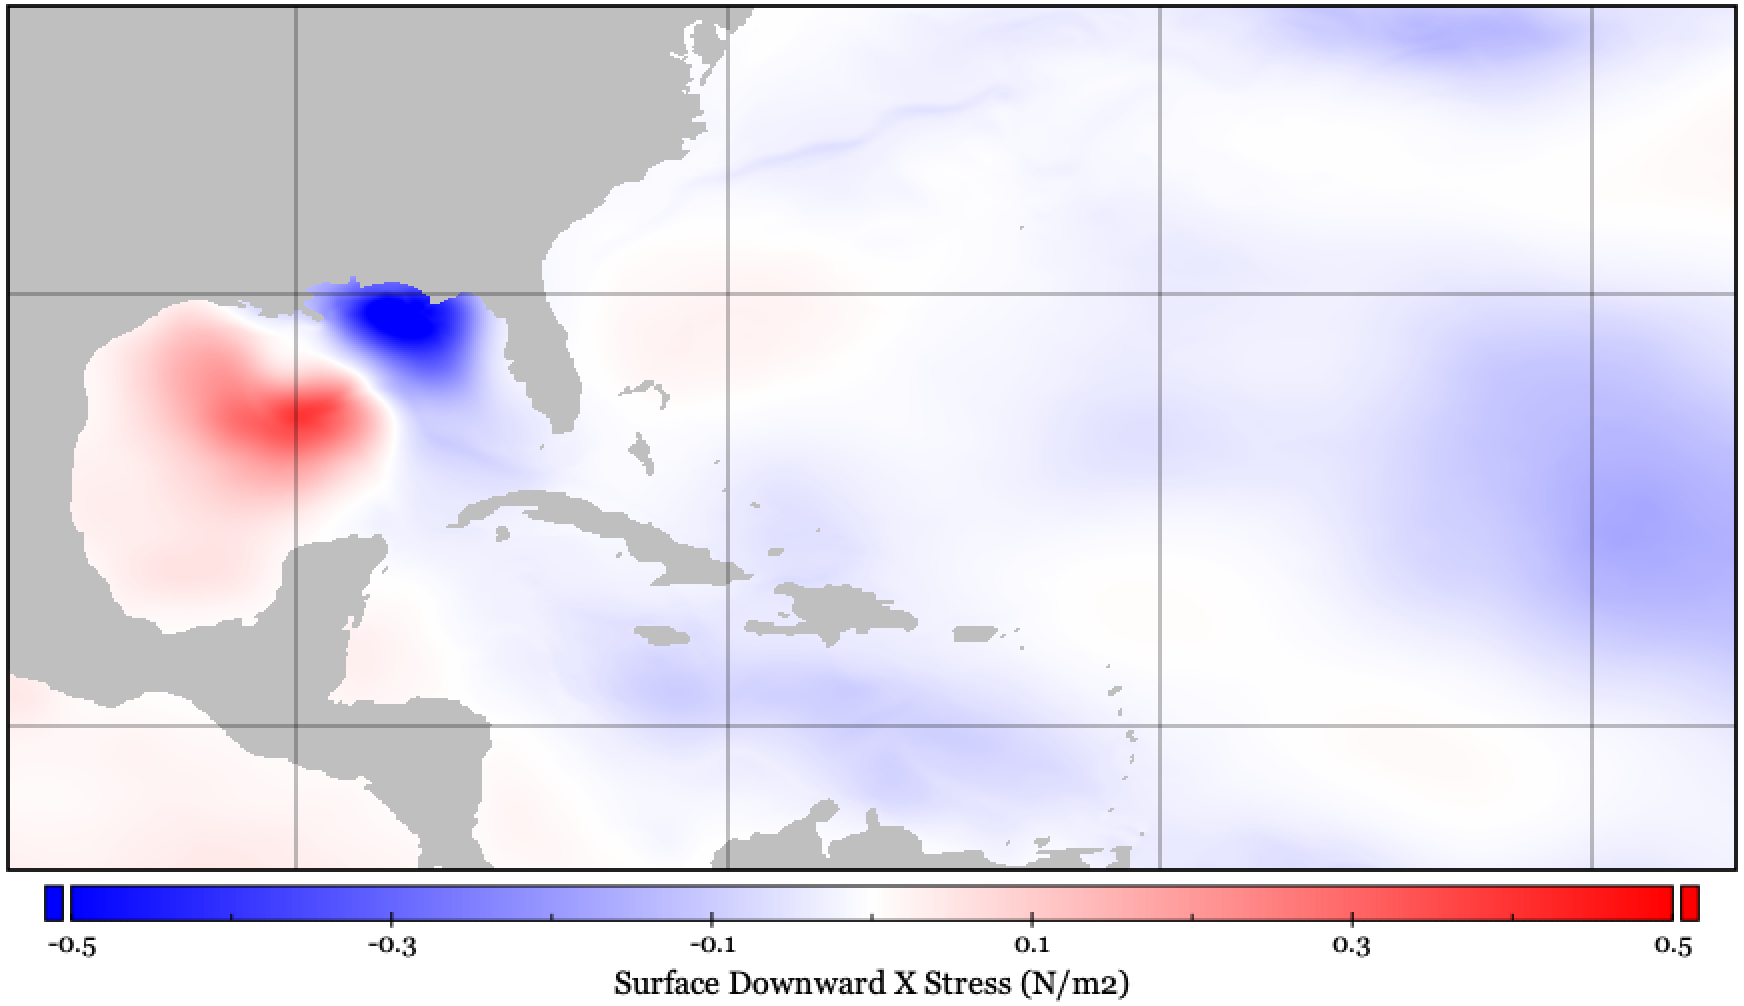
\includegraphics[width=0.93\linewidth]{images/tauuo.png}
      \end{beamercolorbox}
      \vfill
  \end{frame}

\begin{frame}{Yearly $\tau_u$ distributions are similar between 2004/5 }
\vspace{-20pt}
\begin{figure}[htb!]
    \centering
    \includegraphics[width=0.6\linewidth]{../surge/plots/tauuo/stats_points_plot.pdf}
     \hspace{0pt} \includegraphics[width=0.285\linewidth]{../surge/plots/tauuo/stats_points_plot_1.pdf}
    \vspace{-7pt}
    \caption{A comparison between the distributions of $\tau_u$ above geoid (tauuo)
     for the training set (2005) and the test set (2004).}
    \label{fig:}
\end{figure}
\end{frame}


\begin{frame}{No clear difference between 2004/5  }
\vspace{-20pt}
\begin{figure}[htb!]
    \centering
    \includegraphics[width=0.95\linewidth]{../surge/plots/tauuo/stats_points_plot_2.pdf}
    \vspace{-7pt}
    \caption{$\tau_u$.}
    \label{fig:}
\end{figure}
\end{frame}

\begin{frame}{$\tau_u$ }
\vspace{-20pt}
\begin{figure}[htb!]
    \centering
    \includegraphics[width=0.95\linewidth]{../surge/plots/tauuo/stats_points_plot_5.pdf}
    \vspace{-7pt}
    \caption{$\tau_u$ There does not seem to be anything wrong with the plots.}
    \label{fig:A}
\end{figure}
\end{frame}


\begin{frame}{$\tau_u$  Covariance and Correlation matrices are similar.  }
\vspace{-20pt}
\begin{figure}[htb!]
    \centering
    \hspace{-10pt}
    \includegraphics[width=0.68\linewidth]{../surge/plots/tauuo/corr_cov.pdf}
     \includegraphics[width=0.16\linewidth]{../surge/plots/tauuo/corr_cov_cbar.pdf}
    \vspace{-7pt}
    \caption{A/B: Covariance matrices for 2004/5.\\
    $\quad\quad\quad\;\;$C/D: Correlation matrices for 2004/5.}
    \label{fig:}
\end{figure}
\end{frame}

% tauvo
\section{Tauvo, $\tau_v$ }
    \begin{frame}[plain]
        \vfill
      \centering
      \begin{beamercolorbox}[sep=8pt,center,shadow=true,rounded=true]{title}
        \usebeamerfont{title}\insertsectionhead\par%
        \color{oxfordblue}\noindent\rule{10cm}{1pt} \\
                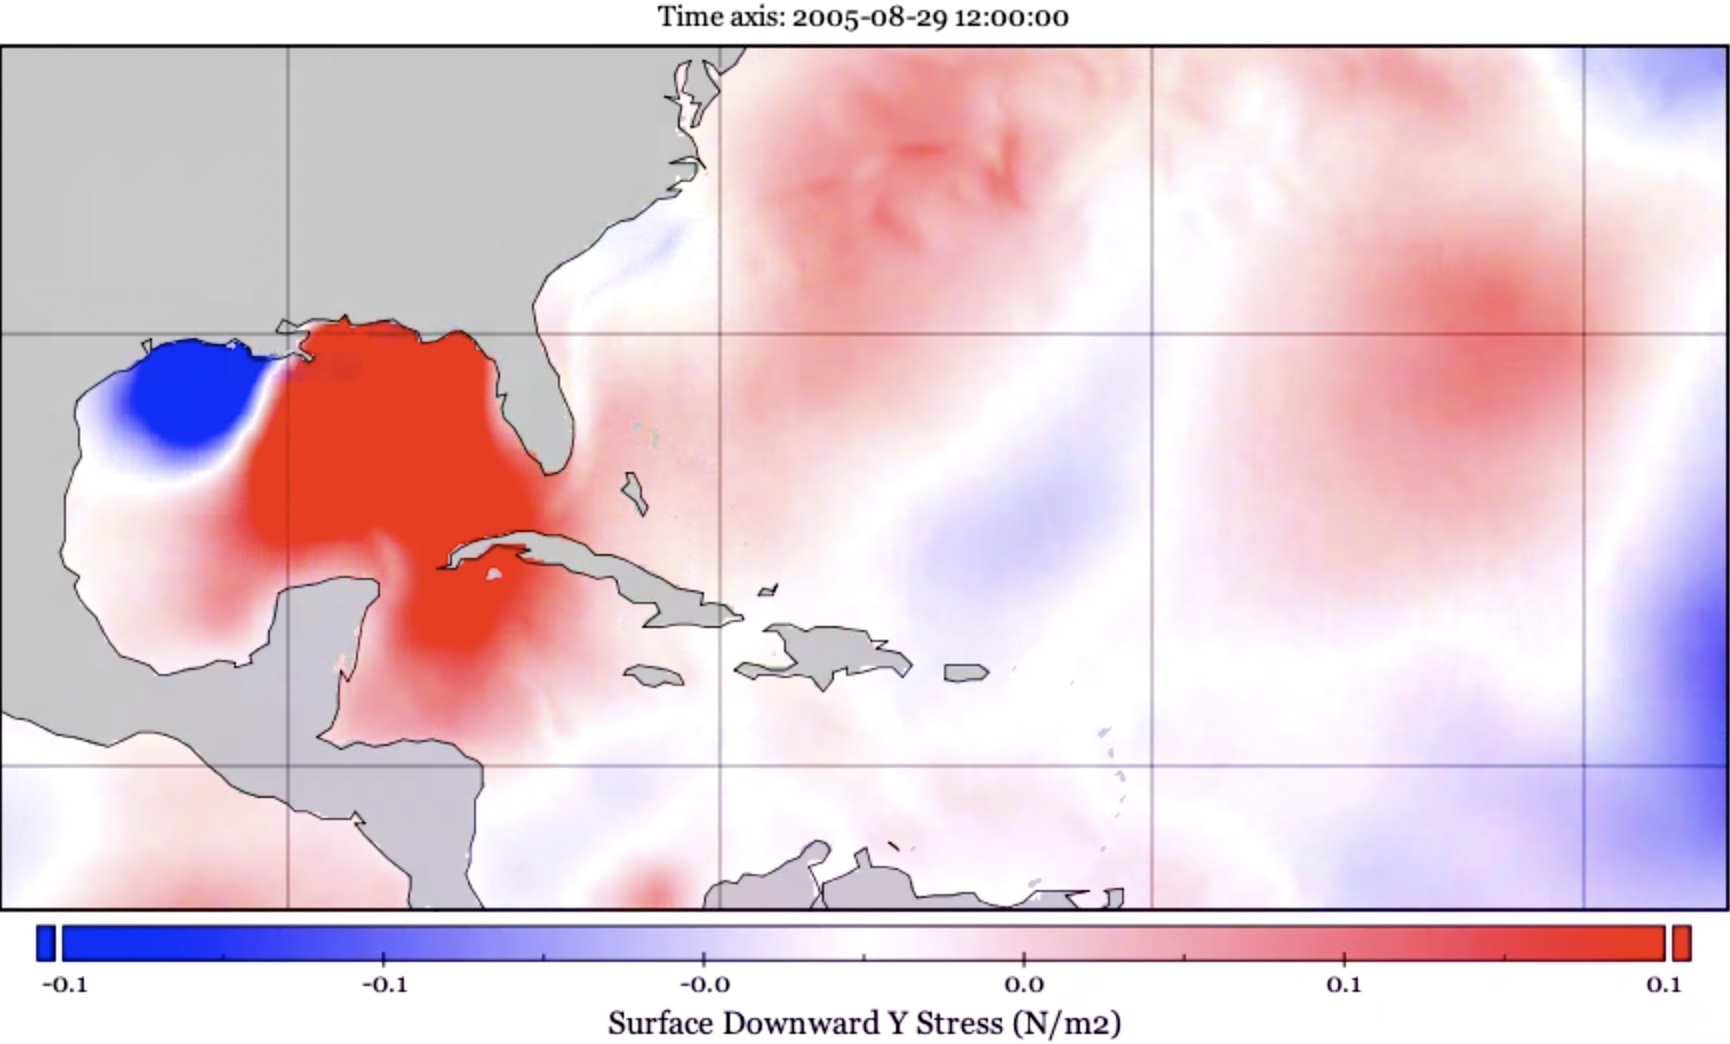
\includegraphics[width=0.93\linewidth]{images/example-images/tauvo.png}
      \end{beamercolorbox}
      \vfill
  \end{frame}

\begin{frame}{$\tau_v$ between 2004/5 }
\vspace{-20pt}
\begin{figure}[htb!]
    \centering
    \includegraphics[width=0.6\linewidth]{../surge/plots/tauvo/stats_points_plot.pdf}
     \hspace{0pt} \includegraphics[width=0.285\linewidth]{../surge/plots/tauvo/stats_points_plot_1.pdf}
    \vspace{-7pt}
    \caption{A comparison between the distributions for
             the training set (2005) and the test set (2004).}
    \label{fig:}
\end{figure}
\end{frame}


\begin{frame}{$\tau_v$  No clear discontinuity between 2004/5  }
\vspace{-20pt}
\begin{figure}[htb!]
    \centering
    \includegraphics[width=0.95\linewidth]{../surge/plots/tauvo/stats_points_plot_2.pdf}
    \vspace{-7pt}
    \caption{}
    \label{fig:}
\end{figure}
\end{frame}

\begin{frame}{$\tau_v$ Mean of Points. }
\vspace{-20pt}
\begin{figure}[htb!]
    \centering
    \includegraphics[width=0.95\linewidth]{../surge/plots/tauvo/stats_points_plot_5.pdf}
    \vspace{-7pt}
    \caption{}
    \label{fig:A}
\end{figure}
\end{frame}


\begin{frame}{$\tau_v$ Covariance and Correlation matrices are similar.  }
\vspace{-20pt}
\begin{figure}[htb!]
    \centering
    \hspace{-10pt}
    \includegraphics[width=0.68\linewidth]{../surge/plots/tauvo/corr_cov.pdf}
    \includegraphics[width=0.16\linewidth]{../surge/plots/tauvo/corr_cov_cbar.pdf}
    \vspace{-7pt}
    \caption{A/B: Covariance matrices for 2004/5.\\
            $\quad\quad\quad\;\;$C/D: Correlation matrices for 2004/5.}
    \label{fig:}
\end{figure}
\end{frame}

\begin{frame}{Running average period controls convexity measure }
\vspace{-20pt}
\begin{figure}[htb!]
    \centering
    \includegraphics[width=1.0\linewidth]{../surge/plots/angle_deriv.pdf}
    \caption{A 50 point running average may be a useful compromise. }
    % \label{fig:}
\end{figure}
\end{frame}


\begin{frame}{The change in angles along the coastline}
\vspace{-20pt}
\begin{figure}[htb!]
    \centering
    \begin{equation}
\bar{B_i}=\operatorname{arctan} 2\left(\frac{1}{n} \cdot
\sum_{j=i-\lambda}^{j=i+\lambda}  \sin B_{j},\; \frac{1}{n}
 \cdot \sum_{j=i-\lambda}^{j=i+\lambda} \cos B_{j}\right)
\end{equation}
    \includegraphics[width=1.0\linewidth]{../surge/plots/angles_plots.pdf}
    \caption{The angle along the coast can be calculated, and averaged in a couple
     of different ways. The average range is subjective.}
    % \label{fig:}
\end{figure}
\end{frame}

\begin{frame}{Let's see if we can remove sinusoids from the data. }
\begin{equation}
\Delta\eta_i = \eta_i - \bar{\eta_i} \sim a\cdot \sin{(\omega(t + \phi))}
\end{equation}
\vspace{-20pt}
\begin{figure}[htb!]
    \centering
    \hspace{-10pt}
    \includegraphics[width=1.1\linewidth]{../surge/plots/fits/coefficients_of_sine.pdf}
    \vspace{-7pt}
   \caption{Fitting sinusoids to each point along the coast for the years.}
    \label{fig:}
\end{figure}
\end{frame}



\begin{frame}{An Example around Miami}
\vspace{-30pt}
\begin{figure}[htb!]
    \centering
    \includegraphics[width=0.75\linewidth]{../surge/plots/miami_map.pdf}
\end{figure}
\end{frame}


\begin{frame}{An Example around Boston}
\vspace{-30pt}
\begin{figure}[htb!]
    \centering
    \includegraphics[width=0.75\linewidth]{../surge/plots/boston_map.pdf}
\end{figure}
\end{frame}


\section{Initial Responsiveness Regression Results\\
(Inspired by 10c \& 10d in Yin et al.~2020~\cite{ZannaPreprint})}
    \begin{frame}[plain]
        \vfill
      \centering
      \begin{beamercolorbox}[sep=8pt,center,shadow=true,rounded=true]{title}
        \usebeamerfont{title}\insertsectionhead\par%
        \color{oxfordblue}\noindent\rule{10cm}{1pt} \\
        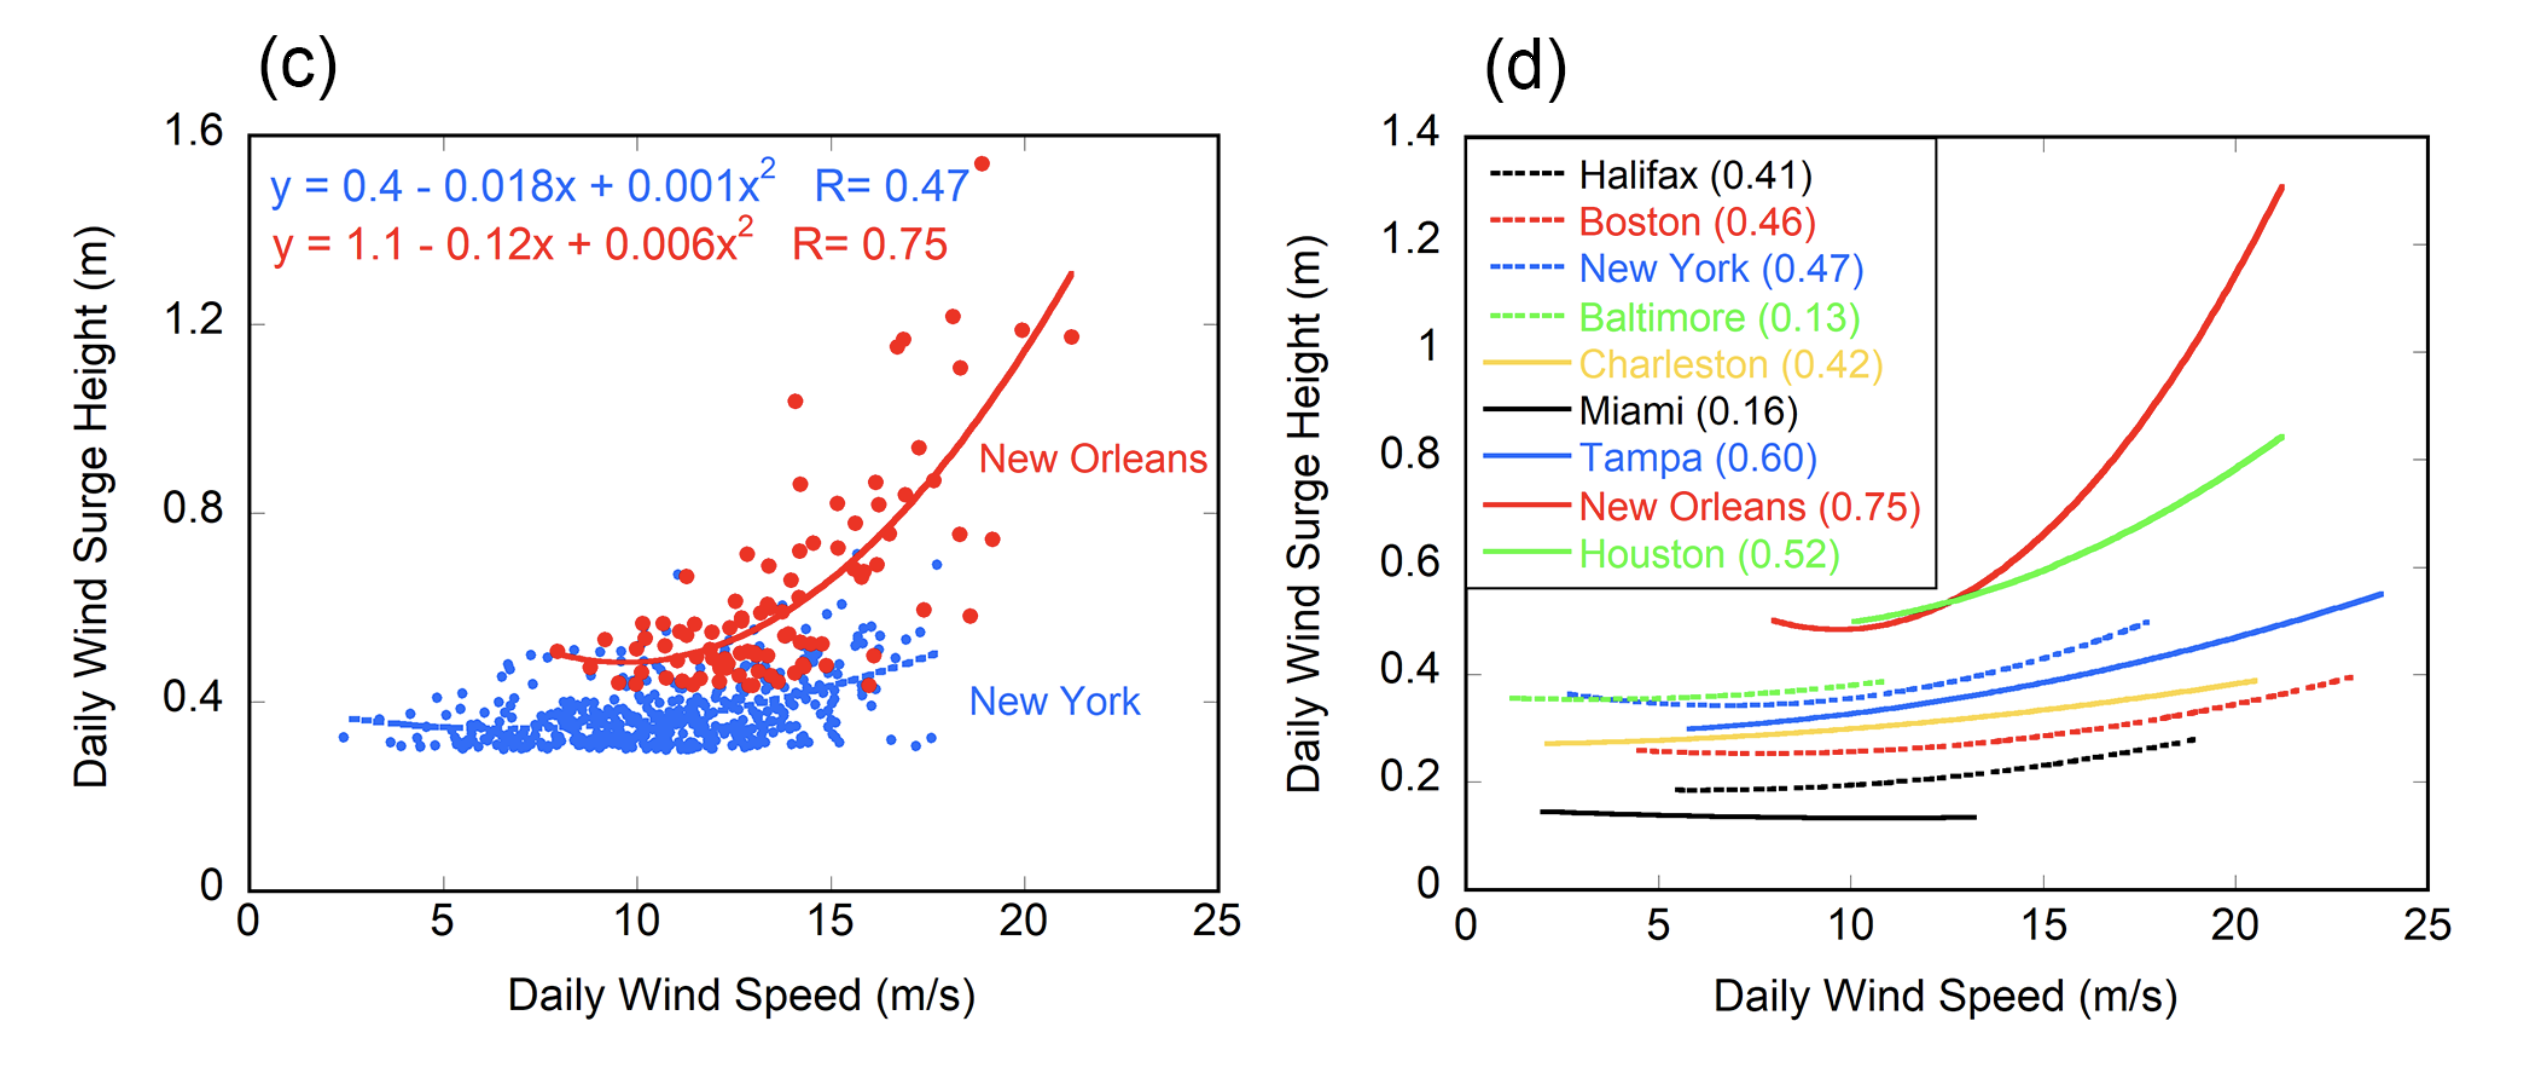
\includegraphics[width=1\linewidth]{images/example-images/yin-responsiveness.png}
      \end{beamercolorbox}
      \vfill
  \end{frame}

\begin{frame}{Thresholding can radically change results  }
\vspace{-20pt}
\begin{figure}[htb!]
    \centering
    \hspace{-10pt}
    \includegraphics[width=0.6\linewidth]{../surge/plots/threshold_plot_new.pdf}
    \vspace{-7pt}
   \caption{Requiring  $\Delta \eta \ge 0$~m is a reasonable criterion,
    and almost maximises the correlation between the wind stress (no location information),
     and threshold at an arbitrary point.}
\end{figure}
\end{frame}

\begin{frame}{Linear Regression of $ \Delta \eta$ against $|U|^2$ for $ \Delta\eta>0$.  }
\vspace{-20pt}
\begin{figure}[htb!]
    \centering
    \hspace{-10pt}
    \includegraphics[width=0.9\linewidth]{../surge/plots/score-plot/score_plot.pdf}
    \vspace{-7pt}
   \caption{Only generalises for the most vulnerable points. Most variance not modelled.}
    \label{fig:}
\end{figure}
\end{frame}

\begin{frame}{Angle derivative $\sigma=15\pm2$ most correlated.   }
\vspace{-20pt}
\begin{figure}[htb!]
    \centering
    \hspace{-10pt}
    \includegraphics[width=1\linewidth]{../surge/plots/check_new.png}
    \vspace{-7pt}
    \caption{$r_p$ with angle derivative against A: training score,
    B: test score, C: linear reg coeff,
    D: $r_p$ of training data.}
    \label{fig:}
\end{figure}
\end{frame}

\begin{frame}{Extracting Bathymetry}
\vspace{-30pt}
\begin{figure}[htb!]
    \centering
    \includegraphics[width=\linewidth]{../surge/plots/simple_bath_extract.pdf}
\end{figure}
\end{frame}

\begin{frame}{Performing Simple Regression }
\vspace{-20pt}
\begin{figure}[htb!]
    \centering
    \hspace{-10pt}
    \includegraphics[width=1\linewidth]{../surge/plots/reg_ready.pdf}
    \vspace{-7pt}
    \label{fig:}
\end{figure}
\end{frame}

\begin{frame}{MLR }
\vspace{-20pt}
\begin{figure}[htb!]
    \centering
    \hspace{-10pt}
    \includegraphics[width=1\linewidth]{../surge/reg_look.pdf}
    \vspace{-7pt}
   \caption{$r_p =0.29$, $r_p =-0.48$, &  $r_p=0.06$. MLR r$^2$=0.308.   }
    \label{fig:}
\end{figure}
\end{frame}


\begin{frame}{$\sigma$ choice}
\vspace{-20pt}
\begin{itemize}
\item Great stuff. Is $\sigma = 10$ a good value?
% \item Chosen based on kurtosis plots (see later) by an NNN (me).
\end{itemize}
\vspace{-10pt}
% 'check_similarity'
\begin{figure}[htb!]
    \centering
    \includegraphics[width=1\linewidth]{../surge/plots/check_similarity.pdf}
   \caption{A: Mean, B: Std Dev, C: Skew, D: Kurtosis.}
    % \label{fig:}
\end{figure}
\vspace{-20pt}
\begin{itemize}
\item Maybe. $\sigma=15\pm2$ leads to the highest $r_p$ against
      the points standard deviation for the year.
\end{itemize}
\end{frame}
